\documentclass[10pt]{article} 
\usepackage[spanish,activeacute]{babel} %idioma español
\usepackage[utf8]{inputenc}             %transforma los tildes a lenguaje latex automáticamente
\usepackage{multirow}                   %Permite cosntruir tablas en las que algunas celdas ocupan varias filas dentro de un entorno tabular con la orden \multirow, en el caso de columnas es \multicolumn  ... \multirrow{nrow}{width}[vmove]{contenido}
% nrow: número de filas a agrupar
%width: ancho de la columna
%vmove: sirve para subir o bajar el texto (opcional)
\usepackage{epsfig}                     %permite incluir gráficos eps
\usepackage{graphicx}                   %Permite incluir gráficos e imágenes
\usepackage{subfig}                     %Permite hacer subfiguras
\usepackage{amsmath}                    %Extiende el modo matemático
\usepackage{amsthm}
\usepackage{amssymb}
\usepackage{mathrsfs}
\usepackage{hyperref}
\usepackage{colortbl} %Permite agregar color a las tablas
\usepackage{epstopdf}                 %Permite utilizar imagenes en formato eps
\usepackage{float}   %permite indicar la posición de las figuras
\usepackage[left=3cm,right=3cm,top=3cm,bottom=3cm]{geometry}
\renewcommand{\baselinestretch}{1.5}
\parskip=4pt

\usepackage{fullpage}            %%
\usepackage{fancyhdr} 
\usepackage{mdframed}            %%

\setlength{\headheight}{54pt}    %%
\setlength{\headsep}{1em}        %%
\setlength{\textheight}{8.5in}  
\setlength{\footskip}{0.5in} 


\fancypagestyle{firstpage}
{
  \fancyhf{}
  \lhead{
\includegraphics[height=5em]{LogoDFI.jpg}}
  \rhead{FI3104-1 \semestre\\
         Métodos Numéricos para la Ciencia e Ingeniería\\
         Prof.: \profesor}
  \fancyfoot[C]{\thepage}
}

\pagestyle{plain}
\fancyhf{}
\fancyfoot[C]{\thepage}


\newcommand{\semestre}{2016-2}
\newcommand{\profesor}{Valentino González}



\begin{document}

\author{Sergio Leiva M.}
\title{\textbf{Informe Tarea 8}}
\date{}
\maketitle

\thispagestyle{firstpage}


\section{Introducción}
Se pide evaluar un péndulo forzado periódicamente, que esta descrito por la ecuación (\ref{eq_pendulo}), la frecuencia natural de pequeñas oscilaciones del péndulo es $\omega_0$ = g/L pero para oscilaciónes
más grandes, la frecuencia es menor. Se espera, por lo tanto, que el péndulo entre en resonancia para frecuancias de forzamiento levemente menores que $\omega_0$.

\begin{equation}
mL^2\ddot{\phi}=-mgLsen(\phi)+F_0cos(\omega t)
\label{eq_pendulo}
\end{equation}
 
 Se pide que se integre numéricamente la ecuación de movimiento y determine cuál es la frecuencia de forzamiento, $\Omega$, para la cual el péndulo alcanza la máxima amplitiud (después de oscilar muchas veces). En especifico se debe usar el método de \textit{Runge Kutta 4}, es decir, de orden 4.
 
\section{Procedimiento}
 Para resolver el problema se planteo usar el método de \textit{Runge Kutta} de orden 4 para obtener una mayor presición en el cálculo, además de que en el enunciado se solicitó. Las constantes que se usaron debieron quedar en función de los últimos 3 dígitos del Rut, por lo que los valores estan expuestos en la Tabla \ref{tab_valores}. 
 
\begin{table}[H]
\centering
\begin{tabular}{|c|c|}
\hline
Parámetro & Valor \\
\hline
m & 0,930 [kg] \\
\hline
L & 1,913 [m]\\
\hline
$F_0$ & 0,054 [N] \\
\hline
\end{tabular}
\caption{Valores de los parámetros físicos que rigen el problema. Estos dependen de los últimos 3 dígitos del Rut.(RRR=937) }
\label{tab_valores}
\end{table}

 Para la implemantación del algoritmo se usó como base, el código que esta en el demo de \textit{Runge Kutta} que se encuentra en el \textit{GitHub} del curso como \textit{demo-rk}. Aunque el demo este presentado para el método de orden 2, solo se deben agregar 2 funciones para encontrar los términos $k_3$ y $k_4$ que siguen las ecuaciones (\ref{eq_k3}) y (\ref{eq_k4}) y cambiar la función que modifica los parámetros de la función, y, ( en este caso, y= ($\phi,\dot{\phi}$)) con la relación (\ref{eq_paso})
 
 \begin{equation}
k_3=hf(y_n +\dfrac{k_2}{2},t_n+\dfrac{h}{2},)
\label{eq_k3}
\end{equation}

\begin{equation}
k_4=hf(y_n +k_3,t_n+h)
\label{eq_k4}
\end{equation}

\begin{equation}
y_{n+1} = y_{n}+\frac{1}{6}(k_6+2(k_3+k_2)+k_1)
\label{eq_paso}
\end{equation}
 
Algo importante en lo que se tuvo que poner atención es que al contrario del demo, en este problema, existe una dependencia temporal, por lo que se debe tomar distinto a los demas parámetros de la función. En las ecuaciónes (\ref{eq_k3}) y (\ref{eq_k4}) se usan los subindices n, para denotar que son dependientes del paso número n.

Para encontrar la frecuancia de forzaje que lleva a la amplitud máxima (después de oscilar muchas veces), basta con repetir los calculos para un gran número de valores de $\Omega$ y guardar el valor máximo de los $\phi$ y su $\Omega$ asociado.

Implementar las funciones para que acepten una función generica, es simplemente cambiar los parámetros que reciben las funciones antes definidas, para que solo reciban un set de parámetros de cualquier largo. Para usar de buena manera esto, es recomendable usar arreglos de python, por que estos son mas simples de operar que una lista.

\section{Resultados}
 Una vez que se implemento el algoritmo para integrar la ecuación (\ref{eq_pendulo}), a medida que se cambio el valor de la frecuencia de forzaje, se encontro que podia presentar oscilaciones con una onda envolvente, como muestra la primera imagen de la Figura (\ref{img_forz}) lo cual depende de la relación entre el $\Omega$ de forzaje y el $\omega_0$, frecuencia natural del péndulo, en el caso de la primera imagen, se ve el comportamiento cuando ambas frecuencias son distintas. Para el caso de la segunda imagen de la Figura (\ref{img_forz}) vemos el caso en que las frecuancias $\Omega$ y $\omega_0$, sean iguales, en este punto se produce un efecto de resonancia, es decir, el forzaje nunca esta en contra del movimento y siempre esta inyectado energia al péndulo, por lo que su oscilación aumenta el ángulo indefinidamente.  

\begin{figure}[H]
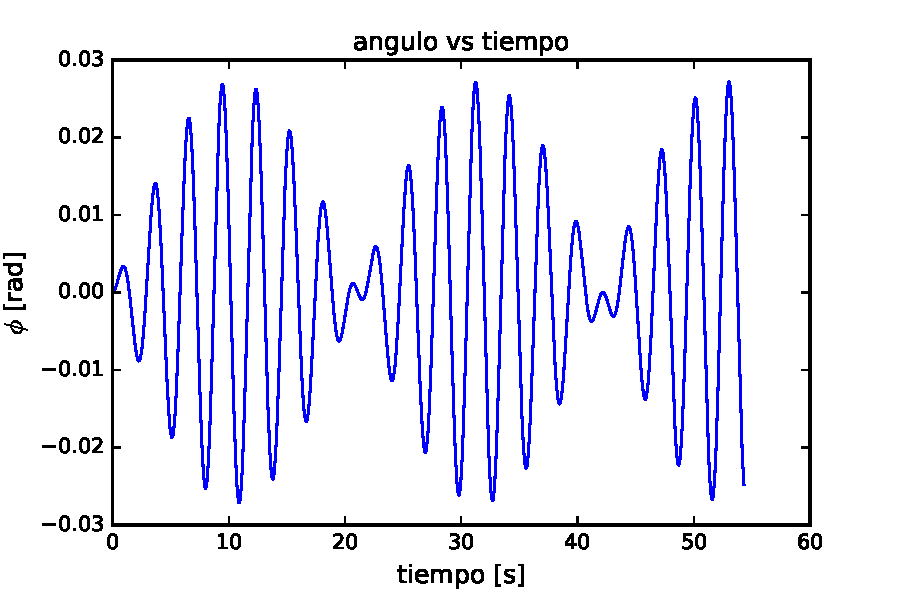
\includegraphics[scale=0.5]{forz_03.pdf}
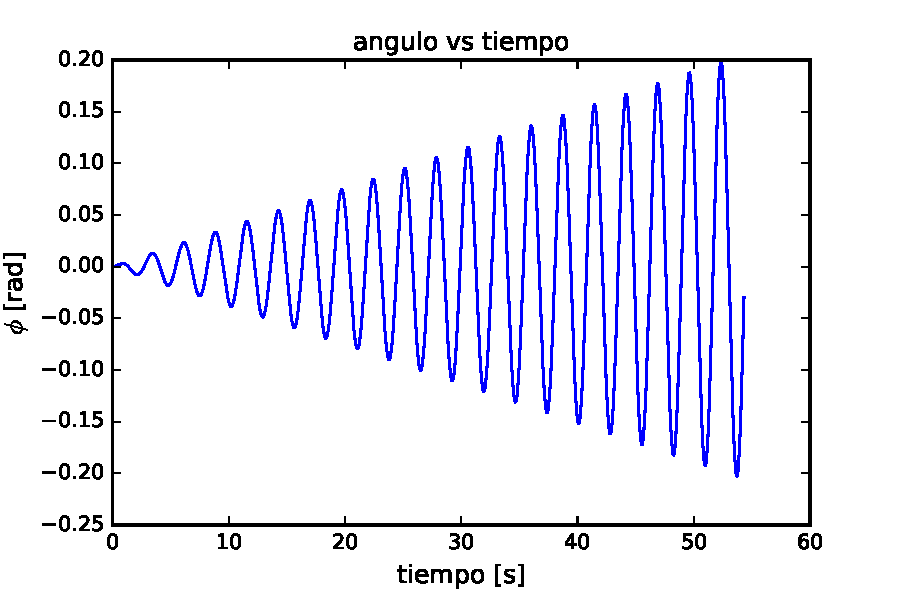
\includegraphics[scale=0.5]{forz_00.pdf}
\caption{La primera imagen muestra el caso en que la frecuencia de forzaje y natural de péndulo sean diferente, y en la seguna imagen se muestra cuando son iguales y se produce una resonancia, potenciando el movimiento de este.}
\label{img_forz}
\end{figure}

 Si bien es cierto que la frecuencia de forzaje no tiene por que tener alguna relación con la frecuancia natural del péndulo, para encontrar un máximo de amplitud, se debio buscar en cercanias al valor de $\omega_0$ tal como se indica el enunciadom dischos máximos deben estar en las cercanias de $\omega_0$ .
\begin{table}[H]
\centering
\begin{tabular}{|c|c|}
\hline
Parámetro & Valor \\
\hline
$\omega_0$ & 2.262 [rad]\\
\hline
$\Omega$ & 2.257 [rad] \\
\hline
\end{tabular}
\caption{Valores de la frecuencia de forzaje ($\Omega$) y la frecuencia de pequeñas oscilaciones ($\omega_0$) del pendulo. El $\Omega$ la frecuencia con cual se obtiene la amplitud máxima.}
\label{tab_omega}
\end{table}


\section{Conclusiones}

 El método de integración de ecuaciones diferenciales, \textit{Runge Kutta} de orden 4 es un método suficientemente confiable y no tan caro computacionalmente, para resolver de manera aceptable un problema relativamente simple. Vistos los gráficos, se comprende que los métodos númericos para resolver ecuaciones diferenciales, son bastante presisos y la intuición para el comportamiento concuerda con lo que obtiene.
 
 Dado que se encontro que las frecuencias tanto de forzaje como natural, son relativamente similares, se puede concluir que el método tiene un buen rango de validez. 
 

\end{document}}